\newpage
\section{Problemática}

La problemática vino dada por la directora de la E.E.S.O N° 214 Mariano Mo-
reno, de Santa Isabel provincia de Santa Fe. Cumpliendo el rol de cliente, planteó
la situación actual respecto al acceso y la seguridad: Las puertas de la institución
no pueden quedar abiertas liberando la entrada, pero no puede destinarse alguien a permitir el acceso de cada persona autorizada fuera de horario o cada persona ex-
terna, por ejemplo el tutor legal de un alumno, ya que muchas veces no hay alguien
en las oficinas de dirección y el personal no docente se encuentra realizando otras
tareas de mantenimiento donde no llega a escuchar el timbre. Adicionando además
el ineficiente tiempo de respuesta de ir a buscar la llave e ir a abrir personalmente
a alguno de los varios puntos de acceso.

\begin{itemize}
    \item Permita el acceso de personal de la escuela (docente y no docente), guardando
registros correspondientes para un control de personal

    \item Permita que una o más personas pertenecientes a la institución habiliten el acceso a un visitante externo desde un dispositivo móvil, identificando al individuo mediante una fotografía.
\end{itemize}

Esto último también controlaría los ingresos fuera de horario, ya que la idea es abrir
las puertas para la entrada regular y restringir el acceso para el horario de clases
fuera de la entrada. Por fuera del horario de las actividades escolares las entradas
quedan bloqueadas con llave.
Es clave en el diseño del sistema el factor económico, ya que el proyecto debe
acotarse al presupuesto de una escuela pública.
Respecto a las particularidades del edificio, este ocupa una manzana completa
el sistema debe controlar tres puntos de acceso. La entrada del patio por la que
acceden los alumnos, la entrada de los docentes y el bicicletero, que también da al
patio exterior donde se dictan las clases de educación física. Las distancias de cada
puerta a la oficina donde se puede colocar un servidor son de 7.5, 3 y 40 metros
respectivamente.

 \begin{figure}[H]
	\centering
	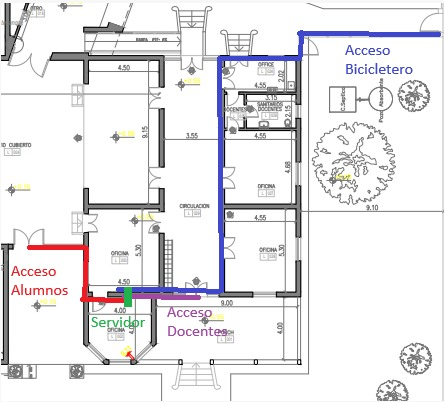
\includegraphics[width=1\textwidth]{img/Plano_Nuevo.jpeg}
	\caption{Plano de la institución resaltando los accesos y ubicación del servidor}
	\label{fig:plano}
\end{figure}

